\subsection{Definition}%
\label{subsec:h-graph_definition}%
Before defining the \ac{h-graph}, some definitions are provided on which the \ac{h-graph} depends. First, recall the \textbf{configuration} definition.\bs

Formally an \textbf{configuration}, $\gls{c}_{id}(k)$ is a tuple of $\left\langle \gls{x}(\gls{k}), \gls{y}(\gls{k}), \gls{theta}(\gls{k})\right\rangle$\\ where $\gls{x}, \gls{y} \in \mathbb{R}, \quad  \gls{theta} \in [0, 2\pi)$\bs

An object is represented as its shape and configuration\\Formally, a \textbf{object},  $\gls{obj}_{id} = \left\langle \gls{objectClass}, \mathit{shape} \right\rangle $\bs

Where \textit{id} is an identifier for the object, \gls{objectClass} the objects classification that can be either movable, unmovable or unknown. $\mathit{shape}$ is linked to a 3D representation of the object.\bs

An object node represents an object in a certain configuration.\\Formally, a \textbf{objectNode}, $V^{\gls{obj}}_{id} =\left\langle \gls{obj}, \gls{c}(k), \textrm{status} \right\rangle $.\bs

Where \textit{id} is an identifier for the node, \gls{obj} an object, $\gls{c}(k)$ the configuration at time step $k$ and status indicates if the configuration is reachable for the object that both reside in the node, the status can be INITIALIZED or COMPLETED or UNFEASIBLE.\bs

An edge describes how a node transitions to another node in the \ac{h-graph}. Edges are split into three categories since they accomplish different goals. \textit{System identification edges} that have as a goal to collect \ac{IO} data and to generate a system model with that data, \textit{action edges} steer a system toward a target configuration and \textit{empty edges} connect nodes that contain different objects that could otherwise not be connected. The edges are formally defined as:\bs

A \textbf{identification edge}, \[\gls{edge}^\mathit{iden}_\mathit{id} = \left\langle \mathit{id_{from}}, \mathit{id_{to}}, \textrm{Identification Method}, \textrm{\ac{IO} data set}, \textrm{controller}, \textrm{system model}, \textrm{status} \right\rangle\]\bs

Where \textit{id} is an identifier for the edge, $\mathit{id_{from}}$ and $\mathit{id_{to}}$ indicating the node identifier where the edge points from and to, respectively.~identification method indicates the used method for system identification, the \textrm{\ac{IO} data set} contains the input sequences and the system's recorded output response, the controller contains the controller used for driving the robot during data collection and the status indicates the node's status that is elaborated in detail in \Cref{tikz:status_identification_edge}.\bs

A \textbf{action edge}, \[\gls{edge}^\mathit{action}_\mathit{id} = \left\langle id_{from}, id_{to}, \textrm{verb}, \textrm{controller},\textrm{system model}, \textrm{path}, \textrm{status} \right\rangle\]\bs

Where \textit{id} is a identifier for the edge, $\mathit{id_{from}}$ and $\mathit{id_{to}}$ indicating the node identifier where the edge points from and to, respectively.~verb is an English verb describing the action the edge represents (in this thesis driving or pushing), the controller contains the control method used for driving the robot, system model is the dynamic system model used by the control method, path is a list of configurations and status indicates the node's status that is elaborated in detail in \Cref{tikz:status_action_edge}.\bs

Connecting nodes with edges is elaborated upon in the upcoming section. Two nodes can only be connected if they both contain the same object. The empty edge main goal is to connect nodes that contain different object, to involve multiple objects in a single action sequence.\bs

A \textbf{empty edge}, \[\gls{edge}^\mathit{emtpy}_\mathit{id} = \left\langle id_{from}, id_{to}, \textrm{status} \right\rangle\]\bs

Where \textit{id} is and identifier for the edge, status for an empty edge can be INITIALIZED or FAILED.\bs

\noindent Now that the nodes and edges have been defined, the \ac{h-graph} can be defined.\bs

Formally, a \textbf{hypothesis graph}, $\gls{h-graph} = \left\langle \gls{nodesH}, \gls{edgesH} \right\rangle $
\\ Where \gls{nodesH} is a set of nodes and \gls{edgesH} a set of edges, defined as:\\ $\gls{nodesH} = \{\gls{nodesH}^{\gls{obj}}_{i}\}$, \quad $\gls{edgesH} \in \{\gls{edge}_{(i,j)}| \gls{edgesH}_i, \gls{edgesH}_j \in \{\gls{nodesH}^{\gls{obj}} \}, i \neq j\}$.\bs

The \ac{h-graph} and most of it's components have been defined. The status of an identification or action edge remains undefined and requires further explanation which is provided in the next subsection.\bs

\subsection{Edge Statuses}\label{subsec:edge_status}
The edges are split into three categories; identification-, action- and empty edges, these edges have just been defined in previous subsection. The status of an identification- and action edge are now defined as \ac{FSM} in \Cref{tikz:status_identification_edge,tikz:status_action_edge}.\bs

\begin{figure}[H]
\centering
\begin{tikzpicture}[node distance = 2cm, auto, initial]
    \node [state, fill=my_dark_blue] (init_test_num) {PrIS\#t};
    \node [state, fill=my_light_blue, below of=init_test_num] (completed_test_num) {PoIS\#t};
    \node [state, accepting, fill=my_green, below of=completed_test_num] (completed) {CO};
    \node [state, accepting, fill=my_red, right of=completed_test_num, node distance=6cm] (failed) {FAIL};

 % arrows
    \draw [-stealth] ([xshift=-2cm]init_test_num.west) to node[near start,above]{\shortstack[]{Select sys.\\ iden. method\\Go to starting pose}} (init_test_num.west);
    \draw[-stealth] (init_test_num) edge[bend right] node[left]{Collect \ac{IO} data} (completed_test_num)
(completed_test_num) edge node[left]{Create system model} (completed);
    \draw [-stealth] (completed_test_num) edge[bend right] node[right]{\shortstack{Go to next\\start configuration}} (init_test_num);
    \draw [-stealth] (completed_test_num) to node[below]{\shortstack[]{Unable to reach next\\start configuration}}  (failed.west);
    % \draw [-stealth] (init_test_num) [out=0, in=90] to node[above]{Unable to reach starting robot configuration}  (failed.north);

\end{tikzpicture}
\caption{\acl{FSM} displaying the status of an identification edge}%
\label{tikz:status_identification_edge}
\end{figure}

\noindent
\begin{table}[H]
\centering
\begin{tabular}%
  {>{\raggedleft\arraybackslash}p{0.30\textwidth}%
   >{\raggedright\arraybackslash}p{0.60\textwidth}}
PRE INPUT SEQUENCE number t (PrIS\#t): & Go to start pose ready to apply the input sequence. \\
POST INPUT SEQUENCE number t (PoIS\#t): & Collect the output response. \\
COMPLETED (CO): & The edge has driven the system toward its target configuration, and its performance has been calculated. \\
FAILED (FAIL): & An error occurred, yielding the edge unusable. \\
\end{tabular}
\end{table}

An identification edge goal is to generate a system model, to then hand over to a corresponding action edge that requires a system model. An action edge's eventual goal is to track a path, to make an action edge ready to track a path or ready for execution a certain number of steps must be completed. First, the existence of a path is estimated, then a system model must be provided, and lastly action planning must be performed. These steps all propagate the status of an action edge as can visualized in \Cref{tikz:status_action_edge}.\bs

\begin{figure}[H]
\centering
\begin{tikzpicture}[node distance = 2cm, auto, initial]
    \node [state, fill=my_purple] (init) {IN};
    \node [state, fill=my_dark_blue, below of=init] (path_exist) {PE};
    \node [state, fill=my_light_blue, below of=path_exist] (system_model) {SM};
    \node [state, fill=my_green, below of=system_model] (path_planned) {PP};
    \node [state, fill=my_yellow, below of=path_planned] (executing) {EX};
    \node [state, accepting, fill=my_orange, below of=executing] (completed) {CO};
    \node [state, accepting, fill=my_red] (failed) at ([xshift=4cm]$(system_model)!0.5!(path_planned)$) {FAIL};

 % arrows
    \draw [-stealth] ([xshift=-2cm]init.west) to node[near start,above]{Select controller} (init.west);
    \draw[-stealth] (init) edge node[left]{Path estimation} (path_exist)
      (path_exist) edge[bend right] node[left]{Load in system model} (system_model)
(system_model) edge[bend right] node[left]{Path planning} (path_planned)
(path_planned) edge[bend right] node[left]{Go to execution loop} (executing)
(executing) edge[bend right] node[left]{Completed} (completed);

    \draw [-stealth] (init.east) [out=0, in=90] to node[xshift=0.1cm, right]{Path non-existence proven}  ([yshift=-0.03cm,xshift=0.2cm]failed.north);
    \draw [-stealth] (path_exist.east) [out=0, in=90] to node[xshift=-0.6cm,yshift=0.55cm, above]{\shortstack[l]{System\\identification\\error}}  ([yshift=-0.03cm,xshift=-0.2cm]failed.north);
    \draw [-stealth] (system_model.east) [out=0, in=180] to node[xshift=0.1cm, yshift=0.3cm, above]{\shortstack[l]{Path\\planning\\error}} (failed.west);
    node[right]{path planning error}
    ([yshift=-0.3cm]failed.west);
    \draw [-stealth] (executing.east) [out=0, in=-90] to node[xshift=0.1cm,right]{Fault detected}(failed.south);

\end{tikzpicture}
\caption{\acl{FSM} displaying the status of an action edge}%
\label{tikz:status_action_edge}
\end{figure}

\noindent
\begin{table}[H]
\centering
\begin{tabular}%
  {>{\raggedleft\arraybackslash}p{0.24\textwidth}%
   >{\raggedright\arraybackslash}p{0.66\textwidth}}
INITIALIZED (IN): & The edge is created between a source and target node.\\
PATH EXISTS (PE): & A graph-based search is performed to validate whether the target configuration is reachable, assuming the system is holonomic. \\
SYSTEM MODEL (SM): & A system model is provided to the controller that resides in the edge.\\
PATH PLANNED (PP): & The path planner plans a path from start- to target configuration. \\
EXECUTING (EX): & The edge receives observations from the robot environment and sends back robot input. \\
COMPLETED (CO): & The edge has driven the system toward its target configuration. \\
FAILED (FAIL): & An error occurred, yielding the edge unusable. \\
\end{tabular}
\end{table}

\paragraph{\ac{h-graph} Legend}
The following figure presents an legend for the \ac{h-graph}s.\bs

\begin{figure}[H]
    \centering
    \begin{subfigure}{0.2\textwidth}
    \centering
    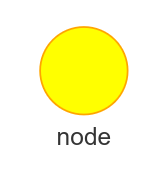
\includegraphics[width=0.7\textwidth]{figures/proposed_method/connecting_nodes/legend/node}
    \caption{Regular node created by the \ac{h-algorithm}.\newline}%
    \end{subfigure}
    \begin{subfigure}{0.2\textwidth}
    \centering
    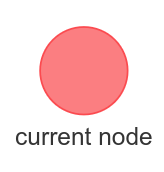
\includegraphics[width=0.7\textwidth]{figures/proposed_method/connecting_nodes/legend/current_node}
    \caption{Current node indicates that its outgoing edge is or is next to be executed.}%
    \end{subfigure}
    \begin{subfigure}{0.2\textwidth}
    \centering
    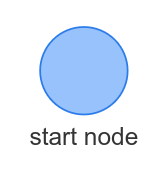
\includegraphics[width=0.7\textwidth]{figures/proposed_method/connecting_nodes/legend/starting_node}
    \caption{Starting node, one is generated at for every subtask.}%
    \end{subfigure}
    \begin{subfigure}{0.2\textwidth}
    \centering
    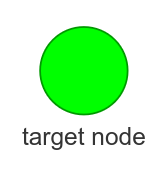
\includegraphics[width=0.7\textwidth]{figures/proposed_method/connecting_nodes/legend/target_node}
    \caption{Target node, one is generated for every subtask.\newline}%
    \end{subfigure}

    \begin{subfigure}{0.33\textwidth}
    \centering
    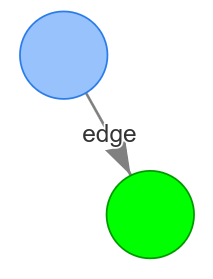
\includegraphics[width=0.7\textwidth]{figures/proposed_method/connecting_nodes/legend/edge}
    \caption{Edge with status IN, PE, SM, PP or EX.}%
    \end{subfigure}
    \begin{subfigure}{0.33\textwidth}
    \centering
    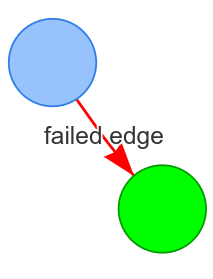
\includegraphics[width=0.7\textwidth]{figures/proposed_method/connecting_nodes/legend/failed_edge}
    \caption{Edge with status FAILED (FAIL)}%
    \end{subfigure}
    \begin{subfigure}{0.33\textwidth}
    \centering
    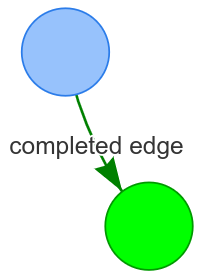
\includegraphics[width=0.7\textwidth]{figures/proposed_method/connecting_nodes/legend/completed_edge}
    \caption{Edge with status COMPLETED (CO)}%
    \end{subfigure}
    \caption{Legend for the \acl{h-graph}. }%
    \label{fig:h-graph_legend}
\end{figure}

The \ac{h-graph} has now fully been defined, in the upcoming section, the \ac{h-algorithm} that creates and updates a \ac{h-graph} is defined and discussed.\bs
